\chapter{Results} 

\section{Genetic Algorithm}

In the following results, each test was ran three times and averaged together to give a better idea of the typical performance of the genetic algorithm approach.  Each test is categorized by the parameter that was changed and the reason and expected results of these parameters is explained.  Also, with the exception of the bitstring segment length test, all other tests are conducted using the normal segment lengths (Table \ref{tab:geneticSegments}).  Lastly, for brevity only the SQL injection results will be compared across all test cases as it is the most complex result out of the three, a full listing of the graphical results for the other two attack types as well as complete text based results for all attack types is included (Appendix \ref{app:fullResults}).

\begin{table}
	\centering
	\label{tab:gaTestParameters}
	\begin{tabular}{|p{1.5in}|p{0.675in}|p{0.675in}|p{0.675in}|p{0.675in}|p{0.675in}|}
	\hline
	\textbf{Test} & \textbf{Popul-ation} & \textbf{Gener-ations} & \textbf{Iter-ations} & \textbf{Muta-tion Rate} & \textbf{Elitist Pool} \\ 
	\hhline{|=|=|=|=|=|=|}
	\textbf{Population Size} & \textbf{$x$} & 100 & 1 & 0.5\% & 5\% \\
	\hline
	\textbf{\# of Generations} & 1250 & \textbf{$x$} & 1 & 0.5\% & 5\% \\
	\hline
	\textbf{Mutation Rate} & 1250 & 100 & 1 & \textbf{$x$} & 5\% \\
	\hline
	\textbf{Eltitist Pool} & 1250 & 100 & 1 & 0.5\% & \textbf{$x$} \\
	\hline
	\textbf{Multiple Iterations} & 1250 & 100 & \textbf{$x$} & 0.5\% & 5\% \\
	\hline
	\textbf{Bitstring Length} & 1250 & 100 & 1 & 0.5\% & 5\% \\
	\hline
	\end{tabular}
	\caption{Parameters used in each Genetic Algorithm Test}
\end{table}

\subsection{Finding Best Parameters}

The performance and effectiveness can often be attributed to the parameters that are used for the genetic algorithm, and there is no universal choice for the parameters as it will depend on your context.  % optimal population size and hte genetic algorithm
Each parameter of the genetic algorithm will affect the results in different ways, therefore it was important to first determine what settings would be most suitable to use for later tests so that the results would not be largely caused by the parameters instead of independent variable in question.  

\subsubsection{Population Size}

Population size is one of the most important parameters as a genetic algorithm with a low population size performs very poorly as there is not a large enough sample size to grow and advance.  Larger populations are more likely to generate new individuals that perform better however this also comes at a performance cost. % cite optimization of control parameters
In addition for our purposes, having a larger population increases the chances of having bitstrings that perform badly as signatures, causing false positives and the like to stick around.  Additionally, in the worst case every attack in the testing set will be unique and require a new signature so a population size any less than that amount may miss attacks.

\begin{figure}
	\label{fig:resPopSize}
	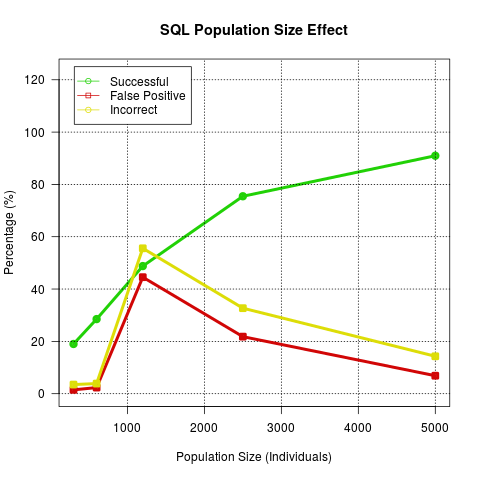
\includegraphics[width=450px]{./assets/results/ga/pop/Results_SQL.png}
	\caption{Effects of Population Size on Detecting SQLi}
\end{figure}

\subsubsection{Generations}

The amount of generations also matters because it is the amount of times the genetic algorithm will run, the more generations the more likely that the algorithm can produce better results and improve upon the old ones.

\begin{figure}
	\label{fig:resGenerations}
	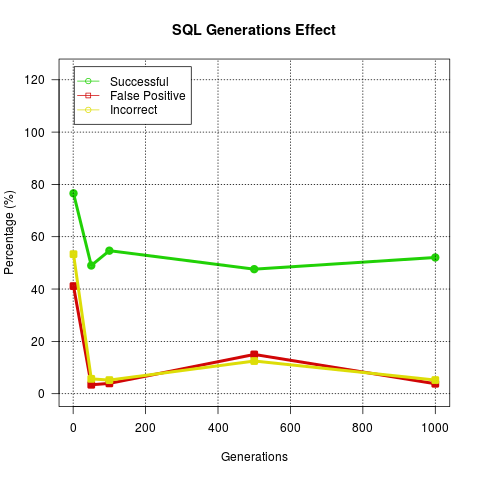
\includegraphics[width=450px]{./assets/results/ga/generations/Results_SQL.png}
	\caption{Effects of Generations on Detecting SQLi}
\end{figure}

\subsubsection{Mutation Rate}

If the mutation rate is too high than the genetic algorithm basically becomes a random search, while no mutation will result in no diversity other than crossovers.  It is very difficult to determine a single mutation rate to get the best results and more often than not this is done by trial and error like the following tests will perform. %cite a new strategy for
Mutation rates are typically set to a very low amount since it is on a per allele basis, a value between 0.0 and 1.0 is often used. % cite optimization of control parameters

\begin{figure}
	\label{fig:resMutation}
	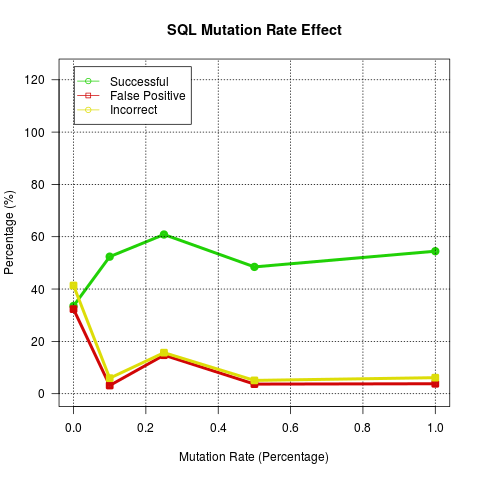
\includegraphics[width=450px]{./assets/results/ga/mutation/Results_SQL.png}
	\caption{Effects of Mutation Rate on Detecting SQLi}
\end{figure}

\subsubsection{Elitist Pool}

The more of the better performing population that survives to the generation the more likely we will have strong individuals to produce newer strong individuals, but if too much of the population is preserved than it may not be able to improve very quickly.  Sometimes this is also referred to as a generation gap. %cite optimization of

\begin{figure}
	\label{fig:resElitist}
	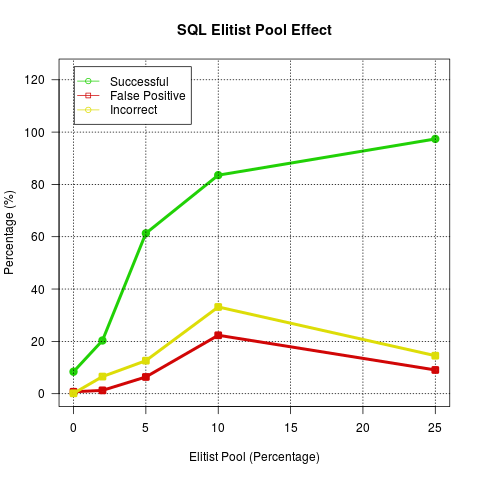
\includegraphics[width=450px]{./assets/results/ga/elitist/Results_SQL.png}
	\caption{Effects of Elitist Pool on Detecting SQLi}
\end{figure}

\subsection{Combining Multiple Signature Sets}

One of the claimed advantages of this approach, and a main reason why it can work is because the genetic algorithm can be used to produce new signatures in order to keep adding to an existing set to increase the detection possibilities.  For this reason, running the algorithm multiple times and combining the signatures should result in more detections, buy may also result in more false positives and incorrect detections.

\begin{figure}
	\label{fig:resIterations}
	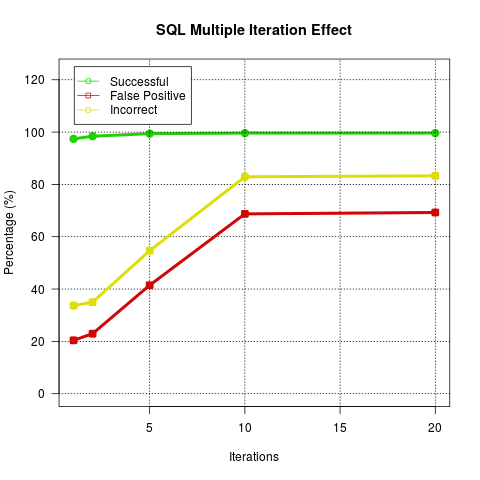
\includegraphics[width=450px]{./assets/results/ga/iterations/Results_SQL.png}
	\caption{Effects of Multiple Iterations on Detecting SQLi}
\end{figure}

\subsection{Bitstring Segment Length Effects}

Because the genetic algorithm can detection new and more attacks by generating new signatures, if the number of possible signatures is less due to the segment length, then it would be more likely to generate these signatures.  However it also opens up the possibility of making it easier to generate bad signatures often.

\begin{figure}
	\label{fig:resLength}
	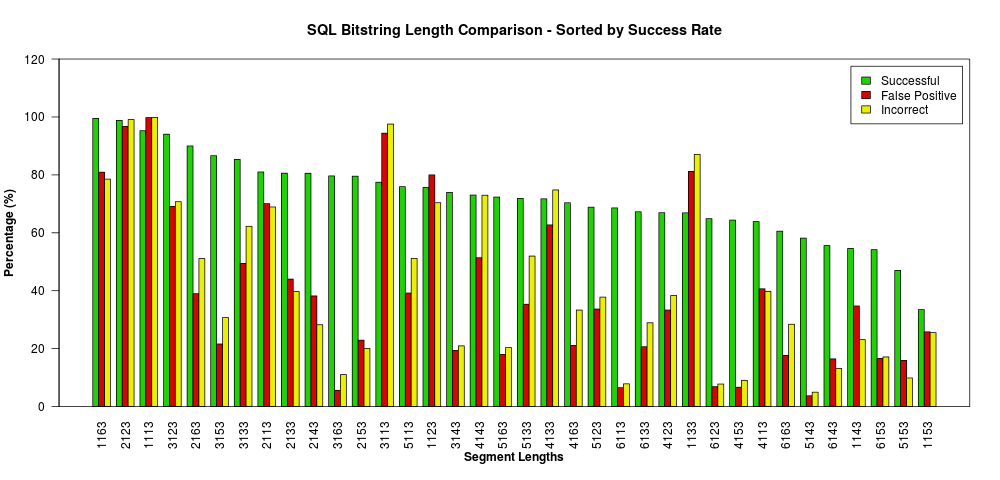
\includegraphics[width=450px]{./assets/results/ga/bitlength/Results_SuccessRate_SQL.png}
	\caption{Effects of Different Segment Lengths on Detecting SQLi}
\end{figure}

\section{Compared With Random Permutations with Fitness}

Because the genetic algorithm is able to increase its detection by generating new signatures automatically, it would be interesting to compare the approach with generating all possible combinations and only using the bitstrings that performed well using the same fitness algorithm used in the genetic algorithm (Algorithm \ref{alg:fitness}).

\begin{figure}
	\label{fig:resRand}
	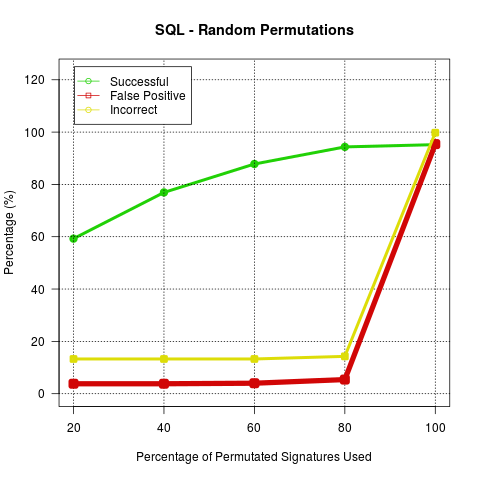
\includegraphics[width=450px]{./assets/results/rand/Results_SQL.png}
	\caption{Permutation of Bitstrings to Detect SQLi}
\end{figure}

\section{Support Vector Machine}

For the support vector machine tests it was not nessecary to average together multiple results as there are no random elements in the approach and the same results are produced everytime.  All results used the same testing data to verify the training process as well as when possible the same training data, so long as the required amount did not exceed the amonut of training data used in the genetic algorithm.  In the genetic algorithm changes can be observed by adjusting parameters, however in the SVM this is not the case and so the amount of training data and what kinds of training data is changed to observe results.

\begin{table}
	\label{tab:svmTestParameters}
	\begin{tabular}{|p{2.0in}|p{1.125in}|p{1.125in}|p{1.125in}|}
	\hline
	\textbf{Test} & \textbf{\# of requests of intended detection type} & \textbf{\# of requests of incorrect detection type} & \textbf{\# of requests of non-attacks} \\ 
	\hhline{|=|=|=|=|}
	\textbf{GA Compairson (30\%/30\%/30\%/10\%)} & \textbf{$x$} & \textbf{$2x$} & \textbf{$y$} \\
	\hline
	\textbf{Increasing Non-Threats} & 300 & 600 & \textbf{$x$} \\
	\hline
	\textbf{Increasing Incorrect-Threats} & 300 & \textbf{$2x$} & 350 \\
	\hline
	\end{tabular}
	\caption{Parameters used in each Support Vector Machine Test}
\end{table}

\subsection{Comparison with Genetic Algorithm}

The first results are using the same training data, as well as the same training proportions used in the genetic algorithm tests of 30\% for each attack type and 10\% of non-threats for the remaining.

\begin{figure}
	\label{fig:resComparison}
	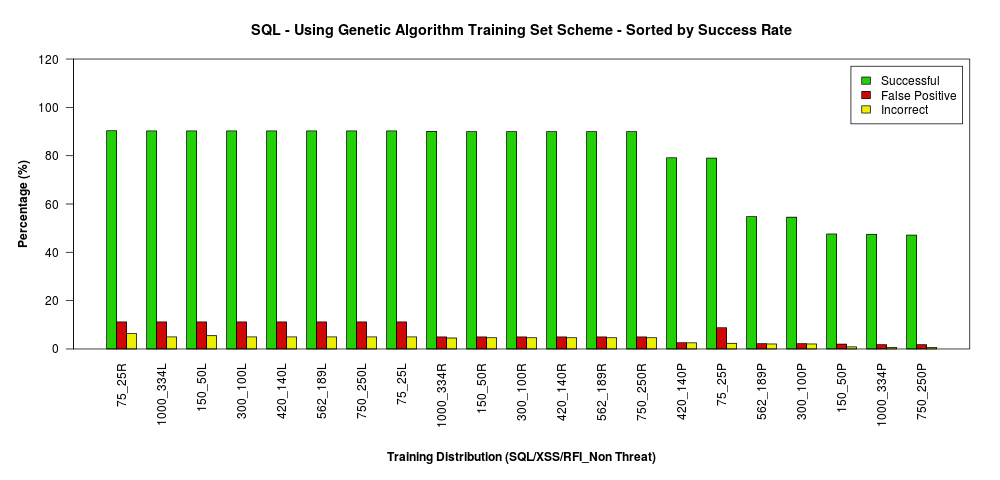
\includegraphics[width=450px]{./assets/results/svm/comparison/Results_SQL.png}
	\caption{Genetic algorithm and SVM comparison for SQLi}
\end{figure}

\subsection{Increasing Non-Threats}

Increasing the amount of nonthreats in the training data should creating a classifier that is more resilient to detecting false positives, the more training data the less likely false positives should occur.

\begin{figure}
	\label{fig:resFalse}
	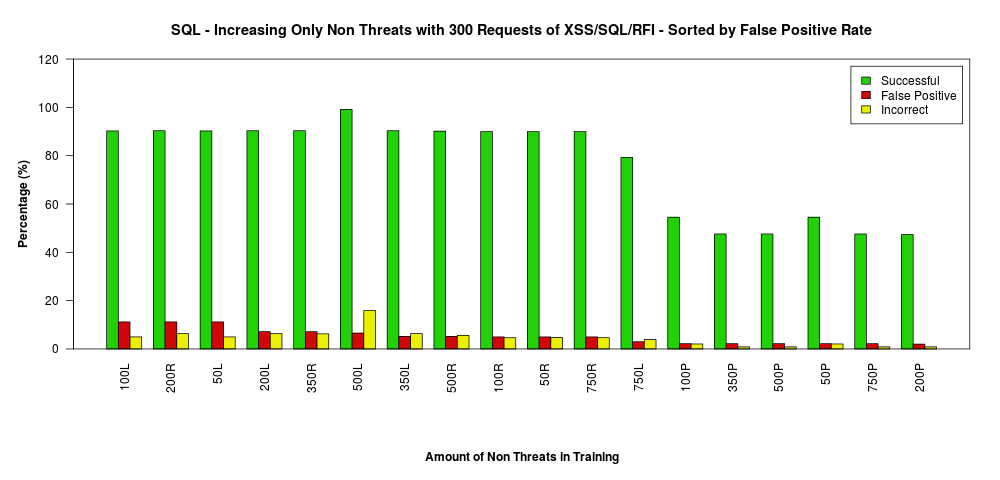
\includegraphics[width=450px]{./assets/results/svm/nonthreat/Results_SQL.png}
	\caption{Effects of increasing non-threat training data in SVM for SQLi detection}
\end{figure}

\subsection{Increasing Incorrect-Threats}

Similar to the last test, the more threats in the training data that are not the one we are looking for, the less likely it is for the classifier to incorrectly identify an attack.

\begin{figure}
	\label{fig:resIncorrect}
	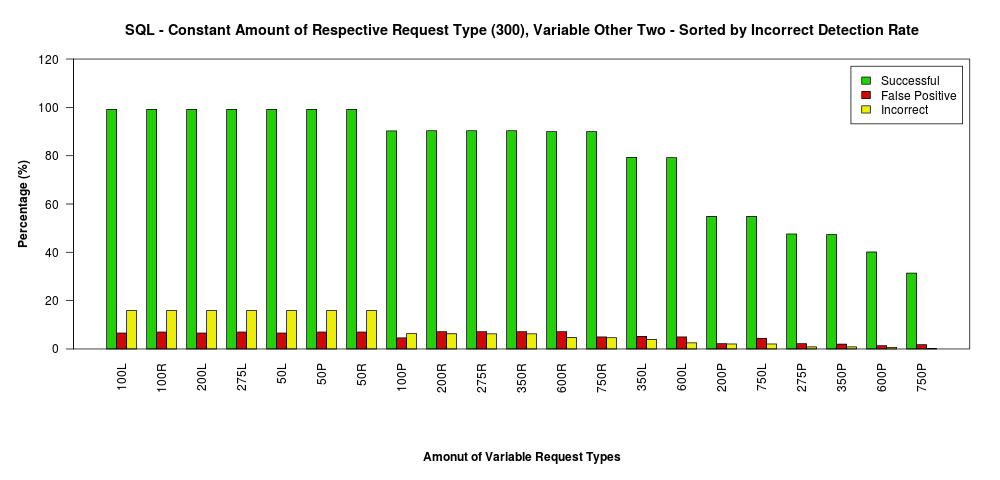
\includegraphics[width=450px]{./assets/results/svm/incorrect/Results_SQL.png}
	\caption{Effects of increasing incorrect attack training data in SVM for SQLi detection}
\end{figure}


